\documentclass[preprint,showkeys,nofootinbib]{revtex4-1}


% linking references
\usepackage{hyperref}
\hypersetup{
  breaklinks=true,
  colorlinks=true,
  linkcolor=blue,
  urlcolor=cyan,
}


% general physics / math packages and commands
\usepackage{physics,amsmath,amssymb,braket,dsfont}
\renewcommand{\t}{\text} % text in math mode
\newcommand{\f}{\dfrac} % shorthand for fractions
\newcommand{\p}[1]{\left(#1\right)} % parenthesis
\renewcommand{\sp}[1]{\left[#1\right]} % square parenthesis
\renewcommand{\set}[1]{\left\{#1\right\}} % curly parenthesis
\newcommand{\bk}{\braket} % shorthand for braket

\renewcommand{\d}{\text{d}}
\newcommand{\g}{\text{g}}
\newcommand{\e}{\text{e}}
\newcommand{\x}{\text{x}}
\newcommand{\y}{\text{y}}
\newcommand{\z}{\text{z}}

\renewcommand{\c}{\hat{c}}
\newcommand{\n}{\hat{n}}

\newcommand{\A}{\mathcal{A}}
\newcommand{\B}{\mathcal{B}}
\newcommand{\D}{\mathcal{D}}
\newcommand{\E}{\mathcal{E}}
\newcommand{\G}{\mathcal{G}}
\renewcommand{\H}{\mathcal{H}}
\newcommand{\I}{\mathcal{I}}
\newcommand{\K}{\mathcal{K}}
\renewcommand{\L}{\mathcal{L}}
\newcommand{\M}{\mathcal{M}}
\newcommand{\N}{\mathcal{N}}
\renewcommand{\O}{\mathcal{O}}
\renewcommand{\P}{\mathcal{P}}
\newcommand{\Q}{\mathcal{Q}}
\renewcommand{\S}{\mathcal{S}}
\newcommand{\U}{\mathcal{U}}

\newcommand{\1}{\mathds{1}}

\newcommand{\mA}{m_{\text{A}}} % symbol for the mass of an atom


% "left vector" arrow; requires tikz package
\newcommand{\lvec}[1]
{\reflectbox{\ensuremath{\vec{\reflectbox{\ensuremath{#1}}}}}}


% figures
\usepackage{graphicx} % for figures
\usepackage{grffile} % help latex properly identify figure extensions
\graphicspath{{./figures/}} % set path for all figures
\usepackage[caption=false]{subfig} % subfigures (via \subfloat[]{})


% inline lists
\usepackage[inline]{enumitem}


% for feynman diagrams
\usepackage{tikz,tikz-feynman}
\tikzset{
  baseline = (current bounding box.center)
}
\tikzfeynmanset{
  compat = 1.1.0,
  every feynman = {/tikzfeynman/small}
}
\newcommand{\shrink}[1]{\scalebox{0.8}{#1}} % for smaller diagrams


% color definitions (used in a figure)
\usepackage{xcolor}
\definecolor{lightblue}{RGB}{31,119,180}
\definecolor{orange}{RGB}{255,127,14}
\definecolor{green}{RGB}{44,160,44}
\definecolor{lightred}{RGB}{214,39,40}

% proper coloring inside math environment
\makeatletter
\def\mathcolor#1#{\@mathcolor{#1}}
\def\@mathcolor#1#2#3{
  \protect\leavevmode
  \begingroup
    \color#1{#2}#3
  \endgroup
}
\makeatother
\newcommand{\bmu}{\mathcolor{lightblue}{\mu}}
\newcommand{\onu}{\mathcolor{orange}{\nu}}
\newcommand{\grho}{\mathcolor{green}{\rho}}
\newcommand{\re}{\mathcolor{lightred}{\text{e}}}


% leave a note in the text, visible in the compiled document
\newcommand{\note}[1]{\textcolor{red}{#1}}

% for strikeout text
% normalem included to prevent underlining titles in the bibliography
\usepackage[normalem]{ulem}


\newcommand{\blue}[1]{\textcolor{blue}{#1}}
\newcommand{\red}[1]{\textcolor{red}{#1}}
\newcommand{\green}[1]{\textcolor{green}{#1}}

% for numbering points in response to referees
\newcounter{point}
\newcommand{\step}{\stepcounter{point}\setcounter{enumi}{0}}


\begin{document}

Dear editors,

In this document, we summarize all revisions made to our manuscript
since its initial submission.  Revisions made in our responses to
Referee 1 (Referee 2) are numbered R1.$X$.$Y$ (R2.$X$.$Y$),
corresponding to the $Y$-th revision in point $X$ of our response.  In
addition, we summarize a few minor revisions made to refine wording or
fix errors in the original manuscript; these revisions are numbered
R3.$Z$.

Excerpts from our original manuscript are written in \red{red}, and
excerpts from the revised version of our manuscript is written in
\green{green}.  All page, line, equation, and reference numbers
generally refer to those in our original manuscript, unless explicitly
stated otherwise.


\section*{Revisions in response to Referee 1}

\setcounter{point}{1}
\begin{enumerate}[label=(R1.\arabic{point}.\arabic*)]

  \step
\item We have inserted a sentence on page 1, line 34:

  \red{... nuclear spin levels.  We fully characterize...}

  which now reads:

  \green{... nuclear spin levels.  Our theory is limited to the
    experimental regime of (i) a deep lattice, with (ii) at most one
    atom occupying each nuclear spin state on any lattice site.  The
    latter restriction is a consequence of initial ground-state
    preparation.  We fully characterize...}


\item The following text on page 4, line 22:

  \red{Specifically, we consider the preparation of isolated few-body
    systems in the deep-lattice limit, ...}

  now reads:

  \green{Specifically, we consider ground-state preparation of
    isolated few-body systems in the deep-lattice limit, ...}


\item We have appended a sentence to the text on page 4, line 31:

  \red{... through the exquisite capabilities with OLCs.}

  which now reads:

  \green{... through the exquisite capabilities with OLCs.  Our theory
    is limited to the experimental regime of at most one atom
    occupying each nuclear spin state on any lattice site, which is a
    consequence of the experimental protocol which starts with all
    atoms in the ground state.}


\item We have rewritten a paragraph on page 4, line 33:

  \red{Though effective multi-body interactions have previously been
    studied in the context of harmonically [35, 36] and
    lattice-confined [37] neutral bosons prepared in a single
    hyperfine state, our work deals for the first time with fermions
    that have internal degrees of freedom and multiple collisional
    parameters.  Nonetheless, due to the SU($N$) symmetry of these
    collisions, we are able to find a simple way to express effective
    multi-body Hamiltonians and fully characterize their low-lying
    many-body energy eigenstates.  While some past work has detected
    experimental signatures of multi-body interactions in the form of
    quantum phase revivals [38], we perform a direct comparison of the
    many-body interaction energies predicted by our low-energy
    effective theory with experimental measurements of
    density-dependent atomic energy spectra performed in ref.~[34],
    similarly to the measurements with bosons performed in ref.~[39].}

  which now reads:

  \green{Though effective multi-body interactions have previously been
    studied in the context of harmonically [35, 36] and
    lattice-confined [37] neutral bosons prepared in a single
    hyperfine state, our work deals for the first time with fermions
    that have internal degrees of freedom and multiple collisional
    parameters.  Some past work has detected experimental signatures
    of multi-body interactions in the form of quantum phase revivals
    [39].  We instead compare the many-body interaction energies
    predicted by our low-energy effective theory to the experimental
    measurements of the density-dependent orbital excitation spectra
    performed in ref.~[34], similarly to the measurements with bosons
    performed in ref.~[38].  To facilitate this comparison of
    excitation spectra and to characterize the low-lying excitations
    in our effective theory, we consider a restriction of our theory
    to states with at most one orbital excitation per lattice site.
    In this case, we find that the SU($N$) symmetry of atomic
    collisions allow the effective multi-body interactions to take a
    remarkably simple form.}


\item We have revised Eq.~(9) and added some discussion, replacing
  (page 7, line 48):

  \red{Our low-energy effective theory exhibits SU($N$)-symmetric
    multi-body interactions, such that the effective interaction
    Hamiltonian can be written in the form
    \begin{align*}
      H_{\t{int}}^{\t{eff}} = \sum_{M=2}^{2I+1} H_M, \tag{9}
    \end{align*}
    where $H_M$ is an $M$-body Hamiltonian, $I$ is the total nuclear
    spin of each atom (e.g.~$I=9/2$ for ${}^{87}$Sr), and the sum
    terminates at $2I+1$ because this is the largest number of atoms
    which may initially occupy a single lattice site.  Focusing on the
    low-lying orbital state excitations of this theory, we find that
    SU($N$) symmetry allows us to express multi-body Hamiltonians in
    the simple form}

  by:

  \green{Our low-energy effective theory exhibits SU($N$)-symmetric
    multi-body interactions, such that the effective interaction
    Hamiltonian can be written in the form
    \begin{align*}
      H_{\t{int}}^{\t{eff}} = \sum_{M=2}^{2I+1} \sum_{p\ge1} H_M^{(p)},
      \tag{9}
    \end{align*}
    where $H_M^{(p)}$ is an $M$-body Hamiltonian of order $p$ in the
    coupling constants $G_X$, and $I$ is the total nuclear spin of
    each atom (e.g.~$I=9/2$ for ${}^{87}$Sr).  The sum terminates at
    $2I+1$ because this is the largest number of atoms which may
    initially occupy a single lattice site.  We explicitly compute all
    of the $M$-body Hamiltonians $H_M\equiv\sum_p H_M^{(p)}$ through
    order $p=3$, yielding effective two-, three-, and four-body
    interactions.  To (i) facilitate a comparison with the
    experimental measurements of many-body orbital excitation spectra
    performed in ref.~[34] and (ii) characterize the low-lying
    excitations in our effective theory, we additionally restrict the
    multi-body Hamiltonians $H_M$ to states with at most one orbital
    excitation per lattice site.  Under this restriction, we find that
    the SU($N$) symmetry of atomic collisions allows us to express all
    multi-body Hamiltonians in the simple form}


\item The text (page 18, line 45):

  \red{Current experiments with ultracold ${}^{87}$Sr on a lattice can
    coherently address ground states and their low-lying orbital
    excitations for up to five atoms per lattice site [34].  Due to
    the SU($N$) symmetry of inter-atomic interactions, manifest in the
    fact that all coupling constants are independent of nuclear spin,
    we can write all effective $M$-body Hamiltonians which address
    these states in the form}

  now reads:

  \green{Current experiments with ultracold ${}^{87}$Sr on a lattice
    can coherently address ground states and single orbital
    excitations of up to five atoms per lattice site [34].  Due to the
    SU($N$) symmetry of inter-atomic interactions, manifest in the
    fact that all coupling constants are independent of nuclear spin,
    a restriction of the $M$-body Hamiltonians $H_M=\sum_p H_M^{(p)}$
    to the subspace of experimentally addressed states takes the form}


\item The text (page 28, line 40):

  \red{Working in the deep-lattice limit, we have derived a low-energy
    effective theory of such atoms.  This theory exhibits emergent
    multi-body interactions that inherit the SU($N$) symmetry of the
    atoms' bare, two-body interactions.  The SU($N$) symmetry of
    $M$-body Hamiltonians in the effective theory has allowed us to
    express them in a simple form, and fully characterize their
    corresponding eigenstates and spectra.}

  now reads:

  \green{Working in the deep-lattice limit and the experimental regime
    of at most one atom occupying each nuclear spin state on any
    lattice site, we have derived a low-energy effective theory of
    these atoms.  Our theory exhibits emergent multi-body interactions
    that inherit the SU($N$) symmetry of the bare two-body
    interactions.  Considering a restriction of our theory to the
    subspace of at most one orbital excitation per lattice site, we
    found that the SU($N$) symmetry of all $M$-body Hamiltonians
    allowed us to express them in a simple form, and to fully
    characterize their eigenstates and spectra.}

\item We have added a considerable amount of text to the beginning of
  section II, such that the opening (page 5, line 19):

  \red{Consider a collection of fermionic atoms with total nuclear
    spin $I$ and two atomic orbital states loaded into a
    translationally invariant 3-D optical lattice.  While an external
    trapping potential will generally break discrete translational
    symmetry of the lattice, any background inhomogeneity can be made
    negligible by spectroscopically addressing a sufficiently small
    region of the lattice [34].  Throughout this paper, we work
    strictly in the deep-lattice regime with negligible tunneling
    between lattice sites.  We also assume a so-called
    ``magic-wavelength'' lattice for which both atomic orbital states
    experience identical lattice potentials [40].}

  now reads:

  \green{The work in this paper is closely tied to the experimental
    work reported in ref.~[34]; we begin with a short summary of the
    relevant experimental procedures therein.  The experiment begins
    by preparing a degenerate gas of $10^4$-$10^5$ (fermionic)
    ${}^{87}$Sr atoms in a uniform mixture of their ten nuclear spin
    states and at $\sim0.1$ of their fermi temperature ($\sim10$
    nanokelvin) [8, 40].  This gas is loaded into a primitive cubic
    optical lattice at the ``magic wavelength'' for which both ground
    (${}^1S_0$) and first-excited (${}^3P_0$) electronic orbital
    states of the atoms experience the same lattice potential [41].
    Lattice depths along the principal axes of the lattice are roughly
    equal in magnitude, with a geometric mean that can be varied from
    30 to 80 $E_{\t{R}}$, where
    $E_{\t{R}}\approx3.5\times2\pi~\t{kHz}$ is the lattice photon
    recoil energy of the atoms (with the reduced Planck constant
    $\hbar=1$ throughout this paper).  These lattice depths are
    sufficiently large as to neglect tunneling on the time scales
    relevant to the experiment.  The temperature of the atoms is also
    low enough to neglect thermal occupation of motional states
    outside the ground-state manifold.}

  \green{Once loaded into an optical lattice, atoms are addressed by
    an external (``clock'') interrogation laser with an ultranarrow
    (26 mHz) linewidth, detuned by $\Delta$ from the single-atom
    ${}^1S_0-{}^3P_0$ transition frequency $\omega_0$.  After a fixed
    interrogation time, the experiment turns off the interrogation
    laser, removes all ground-state (${}^1S_0$) atoms from the
    lattice, and uses absorption imaging to count the remaining
    excited-state (${}^3P_0$) atoms.  Non-interacting atoms in
    singly-occupied lattice sites feature the typical single particle
    lineshape peaked at $\Delta=0$.  The lineshapes of
    multiply-occupied lattice sites, meanwhile, are shifted by
    inter-atomic interactions, which results in spectroscopic peaks
    (i.e.~local maxima in excited-state atom counts) away from
    $\Delta=0$.  A sweep across different detunings $\Delta$ (on the
    scale of inter-atomic interaction energies) thus constitutes a
    measurement of the many-body orbital excitation spectrum.  We note
    that this spectroscopic protocol addresses only singly-excited
    orbital states of lattice sites.  Doubly-excited states are
    off-resonant due to (i) the interaction-induced non-linearity
    ($\sim$kHz) of orbital excitation energies, and (ii) the
    ultranarrow linewidth ($\sim$mHz) of the interrogation laser.}

  \green{While an external trapping potential will generally break
    discrete translational symmetry of the lattice, any background
    inhomogeneity can be made negligible by spectroscopically
    addressing a sufficiently small region of the lattice [34].
    Throughout this paper, we work strictly in the deep-lattice regime
    with negligible tunneling between lattice sites.  We also neglect
    any lattice inhomogeneities and assume that both atomic orbital
    states (i.e.~${}^1S_0$ and ${}^3P_0$) experience identical lattice
    potentials.}


\item To reflect the above change, the text (page 4, line 52):

  \red{In section II we provide an overview of the relevant one- and
    two-body physics of ultracold atoms on a lattice, and summarize
    our main result of effective multi-body interactions between these
    atom.}

  now reads:

  \green{In section II we summarize the experimental procedures
    relevant to our work, provide an overview of the one- and two-body
    physics of ultracold atoms in a deep lattice, and preview our main
    technical results.}


\item We have removed the (now redundant) parenthetical text on page
  5, line 45:

  \red{(with the reduced Planck constant $\hbar=1$ throughout this
    paper)}


  \step
\item We have re-written the paragraph on page 7, lines 20--47:

  \red{We are interested in the ground and low-lying orbital
    eigenstates of several interacting atoms on a single lattice site,
    as such states can be readily prepared and coherently addressed in
    current experiments with ultracold atoms [34].  Although these
    experiments operate at temperatures sufficiently low for
    negligible thermal occupation of excited motional states, simply
    neglecting excited single-particle motional states fails to
    reproduce the observed spectra of multiply-occupied lattice sites.
    The reason for this failure lies in the fact that the bare
    two-body Hamiltonian $H_{\t{int}}$ in (7) is not diagonal in the
    basis of single-particle motional states.  Even at zero
    temperature, therefore, the presence of excited motional states
    modifies many-body atomic energy spectra when the magnitude of
    off-diagonal elements of $H_{\t{int}}$ approach the scale of
    low-lying single-particle motional state energy gaps.  To address
    this problem, we develop a low-energy effective theory for
    ultracold two-level fermionic atoms on a lattice.  As our work is
    motivated by progress in experiments which initialize all atoms in
    identical (i.e.~ground) orbital and motional states, to simplify
    our theory we assume that any $N$ atoms on a single lattice site
    occupy $N$ nuclear spin states.  Multiple occupation of a single
    nuclear spin state on the same lattice site is initially forbidden
    by fermionic statistics, and subsequently cannot be violated in
    the absence of tunneling and hyperfine coupling.}

  In place of the above paragraph, we now have the text:

  \green{Current experiments with ${}^{87}$Sr can prepare up to five
    atoms in the same (ground) orbital state on a single lattice site,
    and coherently address states with a single orbital excitation per
    lattice site [34].  At ultracold temperatures well below the
    non-interacting motional excitation energies
    $\Delta_n\equiv E_n-E_0$ for $n>0$, atoms only occupy their
    motional ground state in the lattice.  For this reason, it is
    common to map the description of these atoms onto a single-band
    Hubbard model that captures all dynamics within the subspace of
    motional ground states of non-interacting atoms, i.e.~with
    wavefunctions $\phi_{i,0}$.  Interactions, however, modify atoms'
    motional ground-state wavefuctions.  The true motional ground
    state of a collection of interacting atoms is then an admixture of
    the non-interacting motional eigenstates, and a naive Hubbard
    model that assumes atomic wavefunctions $\phi_{i,0}$ will fail to
    reproduce the interacting atoms' orbital excitation spectrum.
    Formally, corrections to the spectrum of interacting atoms can be
    accounted for by a perturbative treatment of far-off-resonant
    terms in the interaction Hamiltonian of (7) that create atoms in
    excited motional states,
    e.g.~$\sim\c_{n\mu s}^\dag \c_{0,\nu t}^\dag \c_{0,\nu r}
    \c_{0,\mu q}$ with $n>0$.  These corrections can be understood
    through interaction-induced {\it virtual} occupation of higher
    bands (i.e.~excited motional states), which becomes relevant as
    more atoms occupy the same lattice site, such that their
    interaction energy becomes non-negligible compared to the motional
    excitation energies $\Delta_n$.}

  \green{In order to recast interaction-induced modifications to
    orbital excitation spectra as corrections to the simple Hubbard
    model (i.e.~computed using the non-interacting ground-state
    wavefunctions $\phi_{i,0}$), we develop a low-energy effective
    theory of interacting AEAs in a deep lattice.  To simplify our
    theory, we assume that any $N$ atoms on a single lattice site
    occupy distinct nuclear spin states.  This assumption applies for
    any experimental protocol in which all atoms are initially
    prepared in their orbital and motional ground states (as e.g.~in
    ref.~[34]).  In this case, multiple occupation of a single nuclear
    spin state on any given lattice site is initially forbidden by
    fermionic statistics.  Subsequent violation of this condition
    cannot occur in the absence of inter-site effects or hyperfine
    coupling between nuclear spin states, as is the case in the
    experiment in ref.~[34].}


\item We have changed the text (page 9, line 45):

  \red{The naive idea of neglecting all excited states and using
    $H_{\t{int}}$ directly to describe the spectrum of single-particle
    motional ground states is thus equivalent to truncating our
    expansion for $H_{\t{int}}^{\t{eff}}$ at first order.}

  to:

  \green{Writing down a single-band Hubbard model that simply neglects
    excited atomic motional states and uses $H_{\t{int}}$ directly to
    describe the orbital spectrum of interacting atoms is thus
    equivalent to truncating our expansion for $H_{\t{int}}^{\t{eff}}$
    at first order.}


  \step
\item Eq.~(10) and the following discussion (page 8, line 10):

  \red{\begin{align*} H_M = \sum_{\abs{\set{\mu_j}}=M} \p{U_{M,\g}
        \prod_{\alpha=1}^M \n_{\mu_\alpha,\g} + U_{M,+} \n_{\mu_1,\e}
        \prod_{\alpha=2}^M \n_{\mu_\alpha,\g} + U_{M,-}
        \c_{\mu_1,\g}^\dag \c_{\mu_2,\e}^\dag \c_{\mu_2,\g}
        \c_{\mu_1,\e} \prod_{\alpha=3}^M \n_{\mu_\alpha,\g}},
      \tag{10}
    \end{align*}
    where $\c_{\mu s}\equiv\c_{0,\mu s}$ is a fermionic annihilation
    operator for an atom in the motional ground state with nuclear
    spin $\mu$ and orbital state $s$;
    $\n_{\mu s}\equiv \c_{\mu s}^\dag \c_{\mu s}$ is a number
    operator; and the sum is performed over all choices of nuclear
    spins $\mu_j$ with $j=1,2,\cdots,M$ for which all $\mu_j$ are
    distinct, or equivalently all choices of $\mu_j$ for which the set
    $\set{\mu_j}$ contains $M$ elements, for a total of
    ${2I+1\choose M}\times\p{M!}$ nuclear spin combinations.  The
    coefficients $U_X$ can be expressed in terms of the coupling
    constants of the bare two-body interaction Hamiltonian (see
    Appendix F).  The key feature of the $M$-body interactions in (10)
    is that they take a form identical to the two-body interactions
    between motional ground-state atoms, but with the addition of
    $M-2$ spectator atoms.}

  now reads:

  \green{\begin{align*}
      H_M = \sum_{\abs{\set{\mu_j}}=M}
      H_2^{(\mu_1,\mu_2)} \prod_{\alpha=3}^M \n_{\mu_\alpha,\g},
      \tag{10}
    \end{align*}
    where $H_2^{(\mu_1,\mu_2)}$ is a two-body Hamiltonian addressing
    atoms with nuclear spin $\mu_1,\mu_2$; and
    $\n_{\mu s}=\c_{\mu s}^\dag\c_{\mu s}$ is a number operator for
    atoms with nuclear state $\mu$ and orbital state $s$.  The sum in
    (10) is performed over all choices of nuclear spins $\mu_j$ with
    $j=1,2,\cdots,M$ for which all $\mu_j$ are distinct, or
    equivalently all choices of $\mu_j$ for which the set
    $\set{\mu_j}$ contains $M$ elements, for a total of
    ${2I+1\choose M}\times\p{M!}$ nuclear spin combinations.  The key
    feature of the $M$-body interactions in (10) is that they
    ultimately take the same form as two-body interactions, but with
    the addition of $M-2$ spectator atoms.}


\item Similarly, Eq.~(42) has been changed from (page 18, line 54):

  \red{\begin{align*}
      H_M = \sum_{\abs{\set{\mu_j}}=M}
      \p{U_{M,\g} \prod_{\alpha=1}^M \n_{\mu_\alpha,\g}
        + U_{M,+} \n_{\mu_1,\e} \prod_{\alpha=2}^M \n_{\mu_\alpha,\g}
        + U_{M,-} \c_{\mu_1,\g}^\dag \c_{\mu_2,\e}^\dag
        \c_{\mu_2,\g} \c_{\mu_1,\e} \prod_{\alpha=3}^M \n_{\mu_\alpha,\g}},
      \tag{42}
    \end{align*}}

  to:

  \green{\begin{align*}
      H_M = \sum_{\abs{\set{\mu_j}}=M}
      \p{U_{M,\g} \n_{\mu_1,\g} \n_{\mu_2,\g}
        + U_{M,+} \n_{\mu_1,\e} \n_{\mu_2,\g}
        + U_{M,-} \c_{\mu_1,\g}^\dag \c_{\mu_2,\e}^\dag
        \c_{\mu_2,\g} \c_{\mu_1,\e}}
      \prod_{\alpha=3}^M \n_{\mu_\alpha,\g},
      \tag{44}
    \end{align*}}


  \step
\item We have inserted the following text between lines 35 and 36 of
  page 6:

  \green{Note that the Hamiltonian in (5) is not the true microscopic
    interaction Hamiltonian of AEAs, but rather a generic form for a
    low-energy effective field theoretic description of two-body
    interactions [17, 21, 35--37, 42--44].  There are therefore two
    important points to keep in mind concerning our use of (5) to
    describe two-body interactions.  First, the use of effective field
    theory generically gives rise to divergences that must be dealt
    with either through regularization, e.g.~of the zero-range
    interaction potential implicitly assumed in the expression of (5)
    [45], or through renormalization of the coupling constants in the
    theory.  We chose the latter approach, as we will in any case find
    it convenient to renormalize the coupling constants in the
    effective theory developed in section III.  The choice of method
    to regulate divergences has no effect on the underlying physics.}

  \green{Second, (5) is only the first term in a low-energy expansion
    of two-body interactions in effective field theory, which
    generally includes additional terms containing derivatives of
    field operators.  Derivative terms correspond to the dependence of
    two-body scattering on the relative momentum $k$ of particles
    involved, with $k\to0$ in the zero-energy limit.  In the present
    case of $s$-wave scattering, the leading dependence of the
    two-body interaction Hamiltonian on the relative momentum $k$ can
    be captured by use of an energy-dependent pseudo-potential, which
    amounts to using a $k$-dependent effective scattering length [46].
    This effective scattering length can be determined by expanding
    the $s$-wave collisional phase shift in powers of the relative
    momentum $k$ [45, 47].  Details of this expansion will depend on
    the characteristic length scale of finite-range interactions.  In
    our work, these corrections to (5) will be relevant only for the
    calculation of two-body interaction energies, appearing at third
    order in the coupling constants $G_X$.  As we are primarily
    interested in $M$-body interactions for $M\ge3$, we defer this
    calculation to Appendix D.  We note that our approach of using an
    unregularized contact potential, renormalizing coupling constants,
    and separately accounting for momentum-dependent scattering is
    essentially the same as the approach used for similar calculations
    in refs.~[35--37].  While this approach does not provide insight
    into the microscopic nature of atomic interactions, it is suitable
    for the phenomenological description of these interactions, and
    particular for our eventual development of a low-energy effective
    theory.}


\item The text (page 12, line 15):

  \red{In general, the sums over excited states in the loop diagrams
    of (15) will diverge [35], which implies the need to renormalize
    the coupling constants in our theory.  Even if these diagrams do
    not diverge, we would like to express the effective two-body
    interactions in terms of net, physically observable two-body
    coupling constants as on the right-hand side of (15), rather than
    in terms of long sums at all orders of the bare coupling
    constants.  We therefore renormalize our coupling constants by
    introducing counter-terms $\tilde G_X$ into the effective
    interaction Hamiltonians via $G_X\to G_X+\tilde G_X$.  The values
    of these counter-terms are fixed by enforcing that $G_X$ is equal
    to the net two-body interaction strength.}

  now reads:

  \green{On physical grounds, the net two-body interaction must
    clearly be finite, but individual sums over the excited states in
    loop diagrams of (15) may generally diverge [35].  These
    divergences ultimately appear due to our use of effective field
    theory to describe inter-atomic interactions in (2), (5), and (7),
    rather than a detailed microscopic description of two-atom
    scattering.  Divergences of this sort are a generic feature of
    field theories, and can be dealt with using standard techniques
    such as renormalization.  We therefore renormalize our coupling
    constants by introducing counter-terms $\tilde G_X$ into the
    interaction Hamiltonian.}


\item The text (page 13, line 24):

  \red{Second, the overview we provided in section II, and
    consequently our result in (17), neglects the effect of
    momentum-dependent two-body scattering. When the effective range
    of momentum-dependent interactions is comparable to the scattering
    lengths $a_X$, as is the case for ultracold ${}^{87}$Sr, these
    interactions are third order in the coupling constants $G_X$. Just
    as the $\O\p{G^2}$ counter-terms do not affect $M$-body
    interactions until next-to-leading order (NLO), the $\O\p{G^3}$
    momentum-dependent interactions do not come into play until next-
    next-leading order (NNLO).}

  now reads:

  \green{Finally, our result in (17) neglects the effect of
    momentum-dependent two-body scattering.  When the effective range
    of interactions is comparable to the scattering lengths $a_X$, as
    is the case for ultracold ${}^{87}$Sr, these momentum-dependent
    effects are third order in the coupling constants $G_X$.  Just as
    the $\O\p{G^2}$ counter-terms do not affect $M$-body interactions
    until next-to-leading order (NLO), the $\O\p{G^3}$
    momentum-dependent terms do not come into play until
    next-next-leading order (NNLO).}


  \step
\item We have replaced the following two paragraphs (page 8, line 36):

  \red{As the bare two-body Hamiltonian $H_{\t{int}}$ is not diagonal
    with respect to single-particle motional states, the problem of
    determining many-body spectra and eigenstates nominally involves
    all motional degrees of freedom of the atoms involved.  If we are
    interested in addressing internal atomic states at zero
    temperature, however, in principle we need only to consider the
    motional ground state associated with each many-body internal
    atomic state.  We can then ignore all excited motional states, as
    they will be neither thermally occupied nor externally
    interrogated.  This procedure makes the many-body problem more
    tractable by greatly reducing the dimensionality of the relevant
    Hilbert space.}

  \red{We denote the space of all internal states of atoms in
    single-particle, non-interacting (multi-particle, interacting)
    motional ground states by $\H_{\t{ground}}^{\t{single}}$
    ($\H_{\t{ground}}^{\t{multi}}$).  For sufficiently weak
    interactions, one can construct a unitary transformation $U$
    acting on the full many-body Hilbert space which rotates
    $\H_{\t{ground}}^{\t{multi}}$ into $\H_{\t{ground}}^{\t{single}}$
    [43].  The unitary $U$ can then be used to construct an {\it
      effective Hamiltonian} $H_{\t{int}}^{\t{eff}}$ on
    $\H_{\t{ground}}^{\t{single}}$ that reproduces the spectrum of
    $H_{\t{int}}$ on $\H_{\t{ground}}^{\t{multi}}$, namely
    $H_{\t{int}}^{\t{eff}}=UH_{\t{int}}U^\dag$.  This method for
    constructing an effective theory is commonly known as the
    Schrieffer-Wolff transformation, named after the authors of its
    celebrated application in relating the Anderson and Kondo models
    of magnetic impurities in metals [44].}

  by:

  \green{The net Hamiltonian $H = H_0 + H_{\t{int}}$ for interacting
    AEAs on a lattice is not diagonal with respect to single-particle
    motional state indices (e.g.~$n\in\mathbb{N}_0^3$).  The problem
    of determining interacting atoms' orbital excitation spectrum
    therefore nominally involves all atomic motional degrees of
    freedom.  At zero temperature, however, each orbital state of a
    collection of interacting atoms is associated with a single
    motional ground state.  In order to compute an orbital excitation
    spectrum at zero temperature, in principle we need to identify
    this motional ground state.  We can then ignore all excited
    motional states, which will be neither thermally occupied nor
    externally interrogated.  Such a procedure would drastically
    reduce the dimensionality of the Hilbert space necessary to
    describe the atoms, thereby greatly simplifying any description of
    the atoms' orbital spectrum and internal (i.e.~nuclear and
    orbital) dynamics.  In practice, however, identifying the motional
    ground states of interacting atoms and writing down a Hamiltonian
    restricted to this subspace is a very difficult process to carry
    out analytically.}

  \green{We denote the motional ground-state subspace of the
    non-interacting Hamiltonian $H_0$ by
    $\H_{\t{ground}}^{\t{single}}$, and the motional ground-state
    subspace of the interacting Hamiltonian $H = H_0 + H_{\t{int}}$ by
    $\H_{\t{ground}}^{\t{multi}}$.  That is, all atomic wavefunctions
    for states within $\H_{\t{ground}}^{\t{single}}$ are described by
    $\phi_{i,0}$, while the atomic wavefunctions for states within
    $\H_{\t{ground}}^{\t{multi}}$ are generally unknown, and are in
    principle determined by minimizing the energy of a state with
    respect to its motional degrees of freedom.  Both
    $\H_{\t{ground}}^{\t{single}}$ and $\H_{\t{ground}}^{\t{multi}}$
    are subspaces of the full Hilbert space $\H_{\t{full}}$.  When
    interactions are sufficiently weak compared to the spectral gap
    $\Delta$ between $\H_{\t{ground}}^{\t{single}}$ and its orthogonal
    complement $\H_{\t{full}}\setminus\H_{\t{ground}}^{\t{single}}$,
    one can identify a particular unitary operator $U$ (acting on the
    full Hilbert space $\H_{\t{full}}$) which rotates
    $\H_{\t{ground}}^{\t{multi}}$ into $\H_{\t{ground}}^{\t{single}}$
    [49].  This unitary $U$ can be used to construct an {\it effective
      Hamiltonian} $H_{\t{eff}} = U H U^\dag$ with two key properties:
    (i) $H_{\t{eff}}$ is diagonal in the same (known) basis as the
    non-interacting Hamiltonian $H_0$, and (ii) the spectrum of
    $H_{\t{eff}}$ on $\H_{\t{ground}}^{\t{single}}$ is identical to
    that of the interacting Hamiltonian $H$ on
    $\H_{\t{ground}}^{\t{multi}}$.  The use of an effective
    Hamiltonian $H_{\t{eff}}$ thus overcomes the need to identify
    $\H_{\t{ground}}^{\t{multi}}$ in order to compute the orbital
    spectrum of $H$ at zero temperature.  This method for constructing
    an effective theory is commonly known as the Schrieffer-Wolff
    transformation, named after the authors of its celebrated
    application in relating the Anderson and Kondo models of magnetic
    impurities in metals [50].}


\item We have replaced the text (page 10, line 19):

  \red{Finally, the effective theory involves no corrections to the
    many-body energy eigenstates.  Including such corrections would
    invalidate the effective theory, which preserves the eigenstates
    of the non-interacting Hamiltonian $H_0$ on
    $\H_{\t{ground}}^{\t{single}}$.}

  by:

  \green{Finally, the effective theory involves no corrections to the
    non-interacting many-body energy eigenstates; the purpose of
    constructing the effective Hamiltonian
    $H_{\t{eff}} = H_0 + H_{\t{int}}^{\t{eff}}$ is to reproduce, on
    the known eigenstates of the non-interacting Hamiltonian $H_0$
    within $\H_{\t{ground}}^{\t{single}}$, the spectrum of the
    interacting Hamiltonian $H = H_0 + H_{\t{int}}$ on
    $\H_{\t{ground}}^{\t{multi}}$.  ``Correcting'' the eigenstates of
    the non-interacting Hamiltonian $H_0$ on
    $\H_{\t{ground}}^{\t{single}}$ thus invalidates the effective
    theory.}


  \step
  \step
\item We have appended the following text to section III D, after
  Eq.~(32) on page 16:

  \green{Note that although (22) is a loop diagram, the associated
    factors $\alpha_3^{(3)}$ and $\alpha_5^{(3)}$ in $H_3^{(3)}$ are
    finite.  At large $n$, atoms become free particles for which $n$
    essentially indexes discrete momentum states.  These atoms thus
    have an energy which asymptotically scales as
    $E_n\sim n^2\equiv n_\x^2+n_\y^2+n_\z^2$.  Furthermore, the
    oscillatory behavior of atomic wavefunctions with increasing
    motional state indices $\ell,m$ implies that the overlap integral
    $K_{\ell m}$ becomes sharply peaked at $\ell\approx m$ as $\ell$
    and $m$ get large.  The asymptotic behavior of $\alpha_3^{(3)}$ at
    large $\ell,m,n$ is therefore
    \begin{align*}
      \alpha_3^{(3)}
      \sim \int \f{\d^3\ell~\d^3m~\d^3n}{\p{\ell^2+m^2}\p{\ell^2+n^2}}
      ~\delta\p{\ell-m}\delta\p{\ell-n}
      \sim \int \f{\d^3\ell}{\ell^4}
      \sim \int_{\ell_{\t{min}}}^\infty \f{\d\ell}{\ell^2}
      \sim \f1{\ell_{\t{min}}},
      \tag{33}
    \end{align*}
    where in the last integral we changed to spherical coordinates,
    and $\ell_{\t{min}}^2$ is the minimum value of $\ell^2$ for which
    (i) the energy $E_\ell\sim\ell^2$, and (ii) the integral
    expression in (33) is a good approximation to the corresponding
    sum in (30).  Note that the introduction of $\ell_{\t{min}}$
    amounts to neglecting a finite number of terms in the sum over
    $\ell,m,n$ in (30), whose contribution to the value of
    $\alpha_3^{(3)}$ is finite.  Convergence of $\alpha_5^{(3)}$ is
    similarly guaranteed by the fact that the overlap integral $K_n$
    does not asymptotically grow with increasing $n$, such that
    $\alpha_5^{(3)}$ asymptotically behaves as
    \begin{align*}
      \alpha_5^{(3)} \sim \int \f{\d^3 n}{n^4}
      \sim \int_{n_{\t{min}}}^\infty \f{\d n}{n^2}
      \sim \f1{n_{\t{min}}},
      \tag{34}
    \end{align*}
    where $n_{\t{min}}$ is defined similarly to $\ell_{\t{min}}$.}


  \step
\item We have replaced the following text (page 12, line 35):

  \red{The values of these counter-terms are fixed by enforcing that
    $G_X$ is equal to the net two-body interaction
    strength. Diagrammatically, this renormalization condition is
    \begin{align*}
      \substack{
        \shrink{
          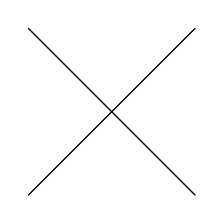
\begin{tikzpicture}
            \begin{feynman}
              \vertex (v);
              \vertex[above left = of v] (f1);
              \vertex[below left = of v] (f2);
              \vertex[above right = of v] (f3);
              \vertex[below right = of v] (f4);
              \diagram* {
                (f1) -- (v),
                (f2) -- (v),
                (v) -- (f3),
                (v) -- (f4) };
            \end{feynman}
          \end{tikzpicture}}
        \\ \O(G)}
      + \substack{
        \shrink{
          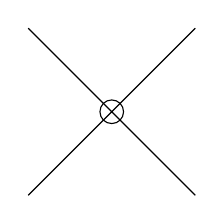
\begin{tikzpicture}
            \begin{feynman}
              \vertex[crossed dot] (v) {};
              \vertex[above left = of v] (f1);
              \vertex[below left = of v] (f2);
              \vertex[above right = of v] (f3);
              \vertex[below right = of v] (f4);
              \diagram* {
                (f1) -- (v),
                (f2) -- (v),
                (v) -- (f3),
                (v) -- (f4) };
            \end{feynman}
          \end{tikzpicture}}
        \\ \O(\tilde G)}
      - \substack{
        \shrink{
          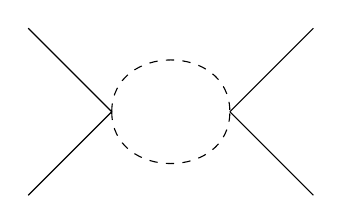
\begin{tikzpicture}
            \begin{feynman}
              \vertex (v1);
              \vertex[above left = of v1] (f1);
              \vertex[below left = of v1] (f2);
              \vertex[right = of v1] (v2);
              \vertex[above right = of v2] (f3);
              \vertex[below right = of v2] (f4);
              \diagram* {
                (f1) -- (v1),
                (f2) -- (v1),
                (v2) -- (f3),
                (v2) -- (f4),
                (v1) --[scalar, half left] (v2),
                (v1) --[scalar, half right] (v2) };
            \end{feynman}
          \end{tikzpicture}}
        \\ \O(G^2)}
      + \cdots = \substack{
        \shrink{
          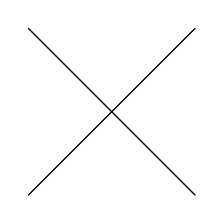
\begin{tikzpicture}
            \begin{feynman}
              \vertex (v);
              \vertex[above left = of v] (f1);
              \vertex[below left = of v] (f2);
              \vertex[above right = of v] (f3);
              \vertex[below right = of v] (f4);
              \diagram* {
                (f1) -- (v),
                (f2) -- (v),
                (v) -- (f3),
                (v) -- (f4) };
            \end{feynman}
          \end{tikzpicture}}
        \\ \O(G)}.
      \tag{16}
    \end{align*}
    where we represent counter-terms by a crossed dot (i.e.~$\otimes$)
    at a vertex. To leading order in the coupling constants, it
    follows that the counter-terms are second order in the coupling
    constants, i.e.~$\tilde G\sim G^2$. This finding implies that
    counter-terms only come into play at next- to-leading order (NLO)
    in the calculation of any effective $M$-body interaction
    Hamiltonian.}

  by:

  \green{The introduction of counter-terms is merely a formal
    decomposition of the ``bare'' coupling constants $G_X^{\t{bare}}$
    that are used in (15) as $G_X^{\t{bare}} = G_X + \tilde G_X$.  In
    performing such a decomposition, we are free to choose the values
    of $G_X$, which in turn fixes the values of
    $\tilde G_X \equiv G_X^{\t{bare}} - G_X$.  For convenience, we can
    choose the values of $G_X$ to be those of the net effective
    coupling constants on the right-hand side of (15).  Representing
    the new coupling constants $G_X$ by regular vertices and the
    counter-terms $\tilde G_X$ by a crossed dot (i.e.~$\otimes$), this
    choice leads to the {\it renormalization condition}
    \begin{align*}
      \substack{
        \shrink{
          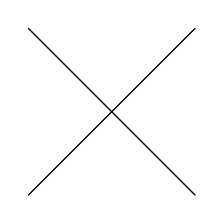
\begin{tikzpicture}
            \begin{feynman}
              \vertex (v);
              \vertex[above left = of v] (f1);
              \vertex[below left = of v] (f2);
              \vertex[above right = of v] (f3);
              \vertex[below right = of v] (f4);
              \diagram* {
                (f1) -- (v),
                (f2) -- (v),
                (v) -- (f3),
                (v) -- (f4) };
            \end{feynman}
          \end{tikzpicture}}
        \\ \O(G)}
      + \substack{
        \shrink{
          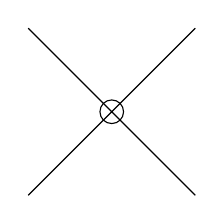
\begin{tikzpicture}
            \begin{feynman}
              \vertex[crossed dot] (v) {};
              \vertex[above left = of v] (f1);
              \vertex[below left = of v] (f2);
              \vertex[above right = of v] (f3);
              \vertex[below right = of v] (f4);
              \diagram* {
                (f1) -- (v),
                (f2) -- (v),
                (v) -- (f3),
                (v) -- (f4) };
            \end{feynman}
          \end{tikzpicture}}
        \\ \O(\tilde G)}
      - \substack{
        \shrink{
          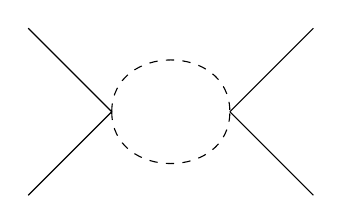
\begin{tikzpicture}
            \begin{feynman}
              \vertex (v1);
              \vertex[above left = of v1] (f1);
              \vertex[below left = of v1] (f2);
              \vertex[right = of v1] (v2);
              \vertex[above right = of v2] (f3);
              \vertex[below right = of v2] (f4);
              \diagram* {
                (f1) -- (v1),
                (f2) -- (v1),
                (v2) -- (f3),
                (v2) -- (f4),
                (v1) --[scalar, half left] (v2),
                (v1) --[scalar, half right] (v2) };
            \end{feynman}
          \end{tikzpicture}}
        \\ \O(G^2)}
      + \cdots = \substack{
        \shrink{
          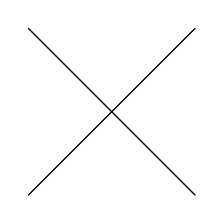
\begin{tikzpicture}
            \begin{feynman}
              \vertex (v);
              \vertex[above left = of v] (f1);
              \vertex[below left = of v] (f2);
              \vertex[above right = of v] (f3);
              \vertex[below right = of v] (f4);
              \diagram* {
                (f1) -- (v),
                (f2) -- (v),
                (v) -- (f3),
                (v) -- (f4) };
            \end{feynman}
          \end{tikzpicture}}
        \\ \O(G)}.
      \tag{16}
    \end{align*}
    This renormalization condition has the benefit of allowing us to
    express effective two-body interactions simply in terms of net
    effective two-body coupling constants, rather than in terms of
    long sums at all order of the bare coupling constants.}


\item The text (page 13, line 17):

  \red{Instead, we must first compute the effective coupling constants
    $G_X^{\t{lattice}}\p{\U}$ in a lattice, which now depend on the
    lattice depth $\U$, and in turn use the effective coupling
    constants to compute interaction energies.}

  now reads:

  \green{The renormalization condition in (16) explicitly fixes $G_X$
    to the net effective coupling constants in any given setting.
    Instead of using free-space coupling constants to compute
    interaction energies in a lattice, we must therefore first compute
    the effective coupling constants $G_X^{\t{lattice}}\p{\U}$, which
    now depend on the lattice depth $\U$, and in turn use these
    effective coupling constants to compute interaction energies.}


\item We have inserted the following paragraph between lines 23 and 24
  on page 13:

  \green{Second, the renormalization condition in (16) implies that
    the counter terms $\tilde G_X$ are second order in the coupling
    constants $G_X$, i.e.~$\tilde G_X\sim G_X^2$.  Although the
    effective Hamiltonian expansions in (13) and (14) are organized in
    powers of the interaction Hamiltonian $H_{\t{int}}$, the couplings
    $G_X$ are the ``small'' parameters in which we can formally
    organize a perturbation theory; more specifically, the formally
    small quantities organizing our perturbation theory are two-body
    ground-state interaction energies (proportional to the couplings
    $G_X$) divided by the spectral gap of the single-atom Hamiltonian
    $H_0$ (see Appendix F).  If $M$ atoms can only couple through
    terms represented by a $p$-vertex diagrams for
    $p\ge p_M^{\t{min}}$, then the leading order contribution to
    $M$-body interactions is order $p_M^{\t{min}}$ in the couplings
    $G_X$.  If the same $p_M^{\t{min}}$-vertex diagrams involve any
    counter-terms, however, then these diagrams are at least order
    $p_M^{\t{min}}+1$ in the couplings $G_X$.  Counter-terms therefore
    only appear at next-to-leading order (NLO) in the calculation of
    effective $M$-body interactions.}


\item The following text (page 13, line 7):

  \red{Before moving on to consider effective three-body interactions,
    there are two comments we must make concerning the result in
    (17).}

  now reads:

  \green{Before moving on to consider effective three-body
    interactions, there are a few comments we must make concerning
    renormalization and the result in (17).}

\end{enumerate}


\section*{Revisions in response to Referee 2}

\setcounter{point}{1}
\begin{enumerate}[label=(R2.\arabic{point}.\arabic*)]
\item
\end{enumerate}


\section*{Miscellaneous revisions}

\begin{enumerate}[label=(R3.\arabic*)]
\item Page 3, line 24 of our original manuscript previously said:

  \red{Last year (2017), a new generation of OLCs became operational
    at JILA}

  Reflecting the fact that it is now 2019, the new version of the
  manuscript says:

  \green{More recently (2017), a new generation of OLCs became
    operational at JILA}


\item Page 5, line 40 of our original manuscript previously said:

  \red{motional state $n\in\mathbb{N}_0^3$ with nuclear spin
    $\mu\in\set{-I,I+1,\cdots,I}$}

  This text contains a sign error; in the version of our manuscript,
  this text reads:

  \green{motional state $n\in\mathbb{N}_0^3$ with nuclear spin
    $\mu\in\set{-I,-I+1,\cdots,I}$}


\item Page 5, lines 43-44 of our original manuscript previously said:

  \red{In a harmonic trap approximation we would have
    $E_n=\p{3/2+n_x+n_y+n_z}\omega$}

  For clarity, we have modified this text so that all subscripts
  denoting free variables (e.g.~the $n$ in $E_n$, as $n$ can here be
  any element of $\mathbb{N}_0^3$) are italic, while all subscripts
  denoting fixed symbols (e.g.~the $x$ in $n_x$, as here $x$ denotes a
  fixed spatial axis) are in roman font.  The new text thus reads:

  \green{In a harmonic trap approximation we would have
    $E_n=\p{3/2+n_\x+n_\y+n_\z}\omega$}

  We have similarly replaced all appearances of $m_A$ (denoting the
  mass of a single atom) with $m_{\text{A}}$; all $E_R$ (denoting the
  lattice photon recoil energy) with $E_{\t{R}}$; all
  $k_L,k_L^x,k_L^y,k_L^z$ (denoting the wavenumber of the lattice
  laser and its projection onto three lattice axes) by
  $k_{\text{L}}, k_{\text{L}}^\x, k_{\text{L}}^\y, k_{\text{L}}^\z$;
  all $\U_x,\U_y,\U_z$ (denoting lattice depths along lattice axes)
  respectively by $\U_\x,\U_\y,\U_\z$; and all
  $T_\mu^z,T_\mu^x,S_{\N X}^z,S_{\N X}^x$ (denoting single-atom and
  many-body pseudospin operators) respectively by
  $T_\mu^\z,T_\mu^\x,S_{\N X}^\z,S_{\N X}^\x$.

  Finally, we have fixed a few discrepancies in our general convention
  that multiple subscripts on a given mathematical symbol should only
  be separated by a comma if at least one of these subscripts has a
  fixed value (as e.g.~in $K^{k\ell}_{mn}$, $K^{\ell,3}_{2,5}$,
  $\c_{\mu n}$, and $\c_{\mu,\g}$).  To this end, we have removed the
  commas on the subscripts ``$M,X$''; ``$N,\pm$''; and ``$\N,\pm$''
  whenever they appear.


\item On page 7, line 17 we previously had the text:

  \red{The existence of such a gauge is guaranteed by the analytic
    properties of Wannier orbitals $\phi_{in}$ [42].}

  With the exception of this sentence, our manuscript has generally
  reserved the word ``orbital'' to refer to electronic degrees of
  freedom of atoms, and ``motional state'' to refer to atoms' spatial
  degrees of freedom.  To avoid potential confusion, we have therefore
  modified the above sentence to read:

  \green{The existence of such a gauge is guaranteed by the analytic
    properties of Wannier wavefunctions $\phi_{in}$ [42].}


\item The last two lines of page 10 and line 26 of page 11 previously
  said:

  \red{Effective $M$-body interaction terms at order $p$ in
    $H_{\t{int}}$ can be represented by directed, weakly connected
    graphs (i.e.~which are connected when ignoring edge direction)
    containing $p$ internal vertices.}

  Though the final expressions in our perturbation theory can indeed
  be represented by weakly connected graphs, intermediate terms that
  cancel out may be represented by graphs that are not connected, as
  e.g.~in Eq.~(35) on page 17.  Furthermore, while the meaning of an
  ``internal vertex'' is likely clear from context, it is better for
  us to define it explicitly.  For clarity, we have therefore modified
  the above text to read:

  \green{Effective $M$-body interaction terms at order $p$ in
    $H_{\t{int}}$ can be represented by directed graphs containing $p$
    vertices with degree greater than one, which we call {\it internal
      vervices}.}


\item To clean up repetitive wording, we have replaced the sentence
  (page 12, line 45):

  \red{To leading order in the coupling constants, it follows that the
    counter-terms are second order in the coupling constants,
    i.e. $\tilde G\sim G^2$.}

  with:

  \green{To leading order, it follows that the counter-terms are
    second order in the coupling constants, i.e.~$\tilde G\sim G^2$.}


\item We fixed an inconsistency in our convention for the ordering of
  operators associated with the coupling symbol
  $G^{\mu q;\nu r}_{\rho s;\sigma t}$.  The text which previously read
  (page 14, line 47):

  \red{for more general
    $\p{\mu,q}+\p{\nu,r}\leftrightarrow\p{\rho,s}+\p{\sigma,t}$
    coupling induced by terms proportional to
    $\c_{\mu q}^\dag \c_{\nu r}^\dag \c_{\sigma t} \c_{\rho s}$.}

  now reads:

  \green{for more general
    $\p{\mu,q}+\p{\nu,r}\leftrightarrow\p{\rho,s}+\p{\sigma,t}$
    coupling induced by terms proportional to
    $\c_{\rho s}^\dag \c_{\sigma t}^\dag \c_{\nu r} \c_{\mu q}$.}

  Both examples are ``correct'' due to the fact that
  $G^{\mu q;\nu r}_{\rho s;\sigma t}$ is self-adjoint, but the latter
  ordering convention is used throughout the rest of the manuscript:
  $G^{\mu q;\nu r}_{\rho s;\sigma t}$ is gives the coupling constant
  for destroying two atoms in state $\p{\mu q}+\p{\nu r}$, and
  creating them in $\p{\rho s}+\p{\sigma t}$.


\item In Eq.~(21), we have fixed an error in the nuclear spin indices
  ($\mu,\nu$) on the two rightmost operators of the middle term, such
  that (page 14, line 53):

  \red{\begin{align*}
      G^{\mu q;\nu r}_{\nu s;\mu t}
      \c_{\nu s}^\dag \c_{\mu t}^\dag \c_{\nu r} \c_{\mu q}
      = -G^{qr}_{ts} \c_{\nu s}^\dag \c_{\mu t}^\dag \c_{\mu r} \c_{\nu q}
      = G^{qr}_{ts} \c_{\mu t}^\dag \c_{\nu s}^\dag \c_{\nu r} \c_{\mu q}.
      \tag{21}
    \end{align*}}

  now reads:

  \green{\begin{align*}
      G^{\mu q;\nu r}_{\nu s;\mu t}
      \c_{\nu s}^\dag \c_{\mu t}^\dag \c_{\nu r} \c_{\mu q}
      = -G^{qr}_{ts} \c_{\nu s}^\dag \c_{\mu t}^\dag \c_{\nu r} \c_{\mu q}
      = G^{qr}_{ts} \c_{\mu t}^\dag \c_{\nu s}^\dag \c_{\nu r} \c_{\mu q}.
      \tag{21}
    \end{align*}}


\item In figure 2 (page 22), all multiplicities (i.e.~values on the
  vertical axes) are integer-valued.  We have therefore adjusted the
  vertical axis on the top left panel of this figure, such that now
  only integer values are marked on this axis.


\item For slight clarification, we have changed the text (page 22,
  line 51):

  \red{... nuclear spins $\mu\in\set{-I,\cdots,I}$ ...}

  to:

  \green{... nuclear spins $\mu\in\set{-I,-I+1,\cdots,I}$ ...}


\item For clarity, we have replaced a few instances of the text
  ``\red{single-particle}'' or ``\red{single-atom}'' by
  ``\green{non-interacting}'' when referring to motional ground states
  of non-interacting particles; specifically, we have done so on page
  9, line 50; on page 11, line 22; on page 13, line 5; and on page 35,
  line 26.


\item To make our first appendix more self-contained, we have defined
  the projector $\P_0$ used therein, such that the text (page 30, line
  38):

  \red{Letting $\Q_0\equiv1-\P_0$ denote the projector onto $\E_0$ and
    $X$ ...}

  now reads:

  \green{Letting $\P_0$ denote the projector onto $\G_0$,
    $\Q_0\equiv\1-\P_0$ denote the projector onto $\E_0$, and $X$ ...}


\item To be more explicit about the restrictions made in Eq.~(F1) in
  Appendix F, we have changed the text (page 40, line 17):

  \red{The $M$-body Hamiltonians addressing low-lying orbital state
    excitations can be writtenin the form}

  to:

  \green{When restricted to the subspace of at most one orbital
    excitation per lattice site, the $M$-body Hamiltonians of the
    low-energy effective theory developed in Section III can be
    written in the form}

  Note that due to the addition of a new appendix in the revised
  version of our manuscript, the above text now appears in Appendix G.


\item Reference 34 of the original manuscript has been published since
  the original submission of our manuscript.  We have updated this
  reference accordingly in the bibliography of our revised manuscript.

\end{enumerate}

\end{document}